% !TeX root = main.tex
\clearpage
\section{Fase 6: Construcción, contenerización y despliegue distribuido}
\label{sec:fase6}
\subsection{B1: Infraestructura multi-nodo}
\label{sec:fase6-b1}

\subsubsection{Topología y recursos asignados}
Se preparó un clúster Docker Swarm de dos máquinas virtuales VMware.
VM-1 mantiene BookStack nativo con Nginx, PHP-FPM y MariaDB; actúa como
manager en estado \texttt{Drain}, para no recibir tareas nuevas. VM-2,
\texttt{cna-node1}, es un clon enlazado y actúa como worker. Se separaron
hostname, machine-id, direcciones MAC y claves de host SSH del clon antes
de incorporarlo al clúster. El usuario Linux \texttt{arqweb} se conserva en
ambas máquinas; no identifica el rol del nodo ni al integrante del equipo.

\begin{table}[H]
\centering\small
\begin{tabularx}{\textwidth}{>{\raggedright\arraybackslash}p{3.1cm}XX}
\toprule
\textbf{Propiedad} & \textbf{VM-1} & \textbf{VM-2} \\
\midrule
Hostname & \texttt{arqwebserver} & \texttt{cna-node1} \\
Procesadores / RAM asignada & 2 vCPU / 4096 MiB & 2 vCPU / 2048 MiB \\
Disco virtual nominal & 20 GB & 20 GB, clon enlazado \\
Red privada, ens37 & \texttt{192.168.145.129/24} & \texttt{192.168.145.130/24} \\
Salida, ens33 & Puente, DHCP & NAT, DHCP \\
Rol Swarm & Manager / Leader / Drain & Worker / Active \\
\bottomrule
\end{tabularx}
\caption{Infraestructura de B1 y asignaciones registradas para la preparación.}
\label{tab:b1-recursos}
\end{table}

La red Solo host conecta Windows y los nodos. Se utiliza la dirección
privada efectiva de VM-1 en las reglas, en lugar de copiar
\texttt{192.168.100.23} de la consigna. Las direcciones obtenidas por DHCP
deben verificarse al cambiar la red o la configuración de VMware; Solo host
no equivale a una reserva de IP. La salida NAT de VM-2 permite instalar
paquetes sin utilizarla como entrada pública de los servicios.

\textbf{Ajuste de recursos:} la captura de creación registra 4 GB iniciales.
Posteriormente se redujo VM-2 a 2048 MiB para compartir el anfitrión con
VM-1. Esta asignación permite preparar el nodo; no demuestra aún que el
conjunto de servicios de B2 quepa bajo carga. Sus límites y presupuesto
agregado se verificarán en B3 antes del despliegue completo.

\clearpage
\subsubsection{Clon enlazado y plataforma de contenedores}
El clon conserva dependencia de sus discos padre; se mantiene esa cadena
de archivos. La elección de clon enlazado y su creación se muestran a
continuación. Las fuentes de los procedimientos se conservan en
\path{cna/deploy/scripts/}; las evidencias originales, en
\path{cna/docs/evidencias/fase6/preparacion/}.

\begin{figure}[H]
\centering
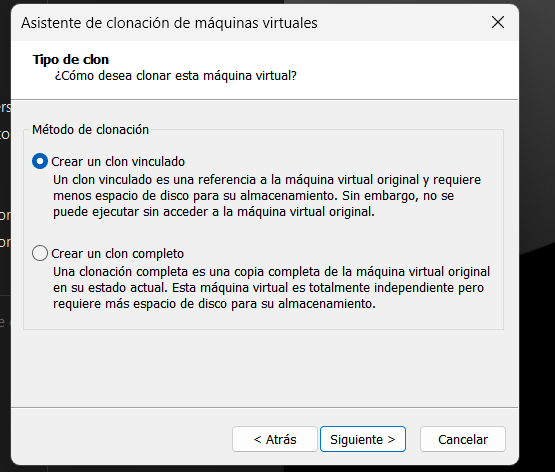
\includegraphics[width=0.52\textwidth,height=5cm,keepaspectratio]{../../../cna/docs/evidencias/fase6/preparacion/PRE-B1-VM2-clon-enlazado.png}
\caption{Preparación B1: selección de clon vinculado en VMware.}
\label{fig:b1-clon-enlazado}
\end{figure}

\begin{figure}[H]
\centering
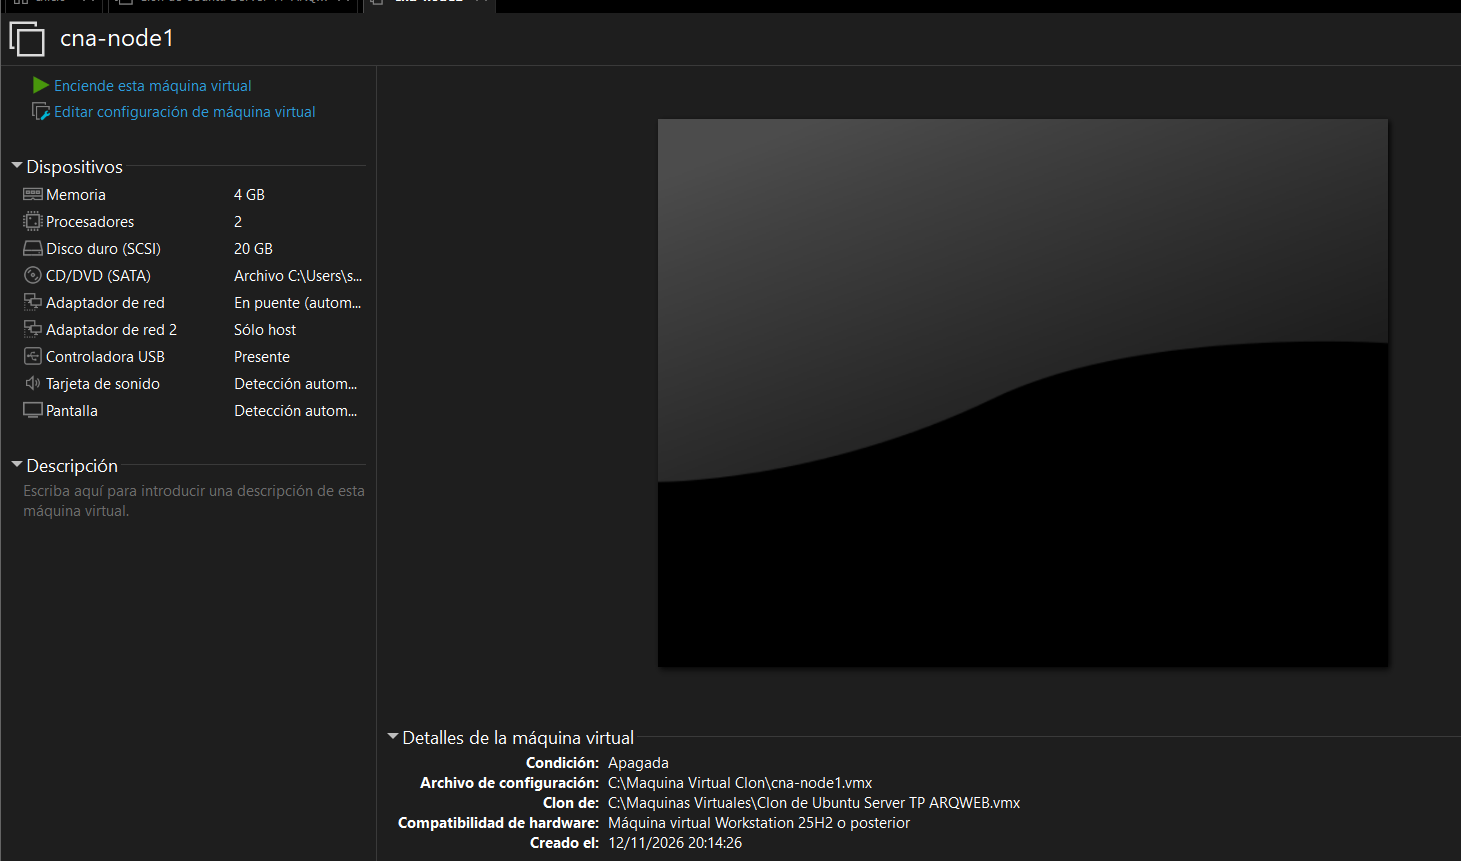
\includegraphics[width=\textwidth,height=8cm,keepaspectratio]{../../../cna/docs/evidencias/fase6/preparacion/PRE-B1-VM2-creada.png}
\caption{VM-2 creada como cna-node1. La captura registra los 4 GB iniciales, anteriores al ajuste a 2 GB.}
\label{fig:b1-vm2-creada}
\end{figure}

\clearpage
En ambos nodos se instalaron Docker Engine Community 29.9.3 y el plugin
Docker Compose v5.7.1. Las capturas de instalación preceden a la formación
del clúster; por ello muestran \texttt{Swarm=inactive}. El estado posterior
y definitivo de los nodos se muestra en F6-E1.

\begin{figure}[H]
\centering
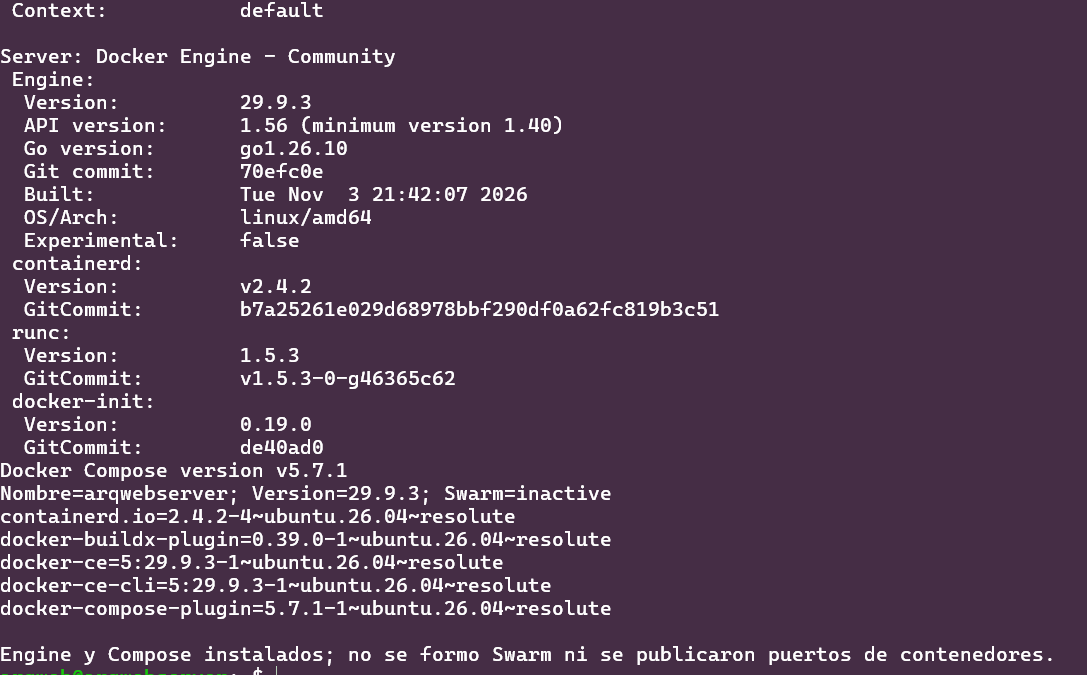
\includegraphics[width=0.84\textwidth,height=6.7cm,keepaspectratio]{../../../cna/docs/evidencias/fase6/preparacion/PRE-B1-VM1-Docker-Compose.png}
\caption{Docker Engine y plugin Compose instalados en VM-1, antes de inicializar Swarm.}
\label{fig:b1-docker-vm1}
\end{figure}
\begin{figure}[H]
\centering
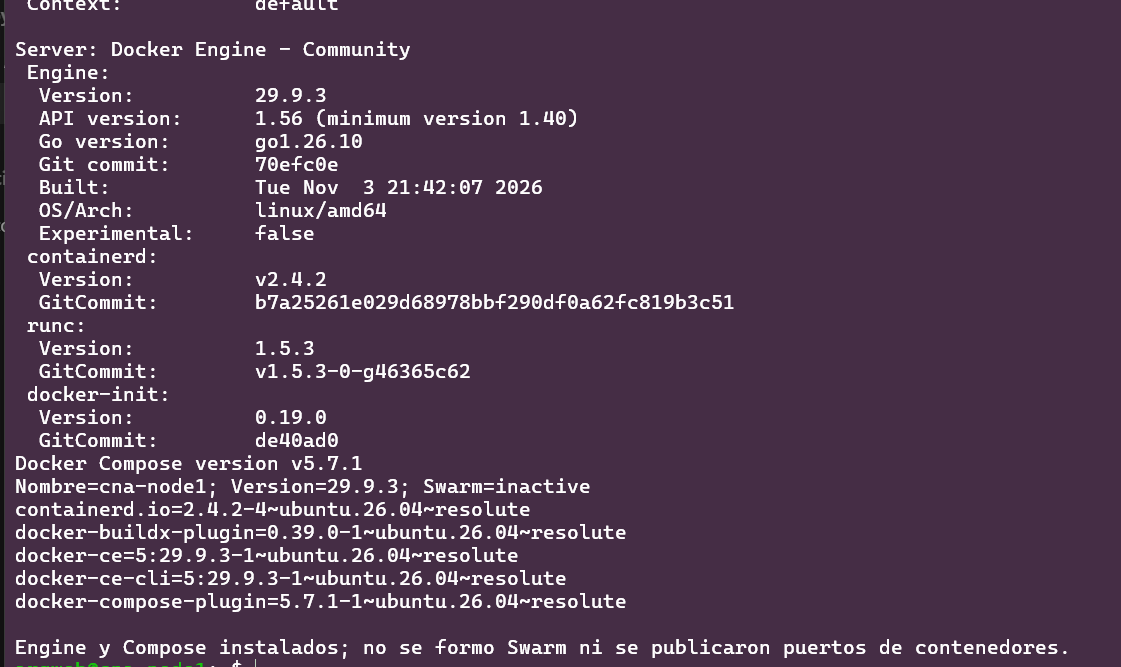
\includegraphics[width=0.84\textwidth,height=6.7cm,keepaspectratio]{../../../cna/docs/evidencias/fase6/preparacion/PRE-B1-VM2-Docker-Compose.png}
\caption{Docker Engine y plugin Compose instalados en VM-2, antes de unir el worker.}
\label{fig:b1-docker-vm2}
\end{figure}
\begin{figure}[H]
\centering
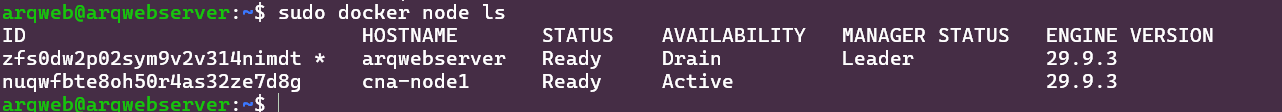
\includegraphics[width=\textwidth]{../../../cna/docs/evidencias/fase6/preparacion/F6-E1-nodos-swarm.png}
\caption{F6-E1 / P33: ambos nodos Ready; VM-1 Leader/Drain y VM-2 Active.}
\label{fig:F6-E1}
\end{figure}

\clearpage
\subsubsection{Firewall por nodo y separación de accesos}
Se mantuvo UFW activo con entrada denegada por defecto. VM-1 conserva
22/TCP para administración, 80/TCP de la configuración HTTP previa y
443/TCP para HTTPS. La entrada funcional de la aplicación permanece en
HTTPS de VM-1. El plano de Swarm solo admite el par privado VM-2 por
\texttt{ens37}: 2377/TCP, 7946/TCP y UDP, y 4789/UDP.

En VM-2 se retiraron las reglas generales de 22, 80 y 443. SSH se permite
desde Windows (\texttt{192.168.145.1}) y VM-1; esta es una excepción de
administración. Los puertos Swarm 7946/TCP y UDP y 4789/UDP solo aceptan
VM-1. Los puertos de servicio futuros deberán admitir únicamente VM-1.

\begin{figure}[H]
\centering
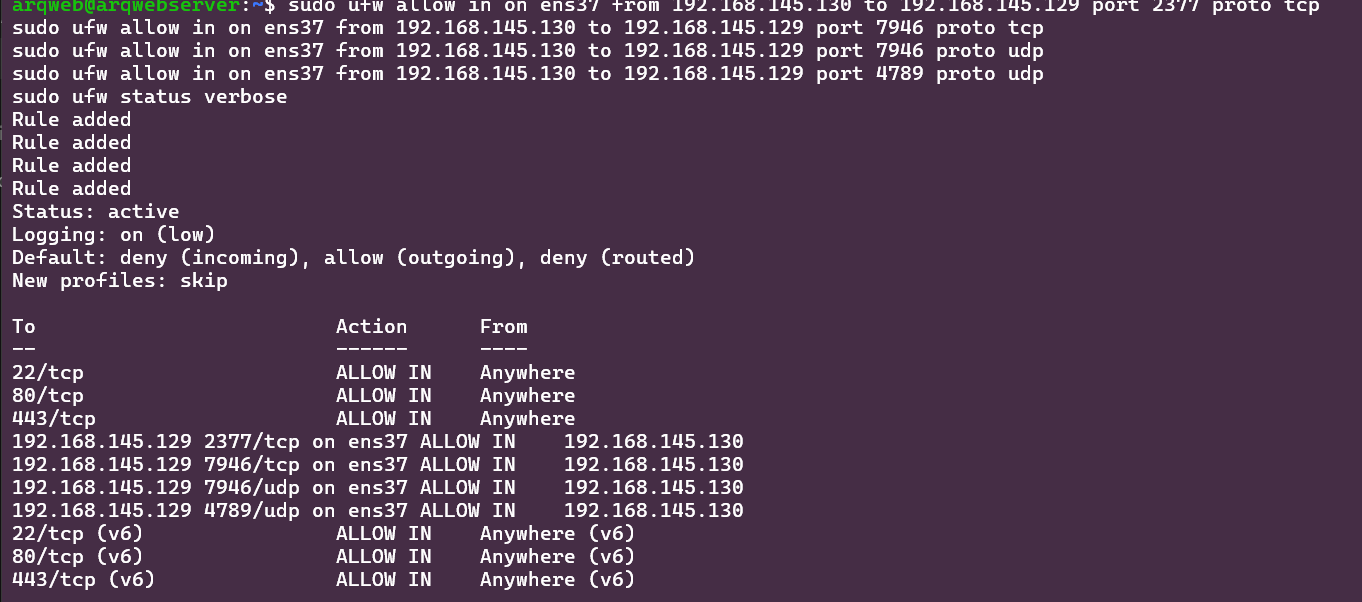
\includegraphics[width=\textwidth,height=9cm,keepaspectratio]{../../../cna/docs/evidencias/fase6/preparacion/PRE-B1-VM1-ufw-Swarm.png}
\caption{F6-E2 / P34, VM-1: política UFW y puertos Swarm limitados a VM-2 por la red privada.}
\label{fig:F6-E2-vm1}
\end{figure}
\begin{figure}[H]
\centering
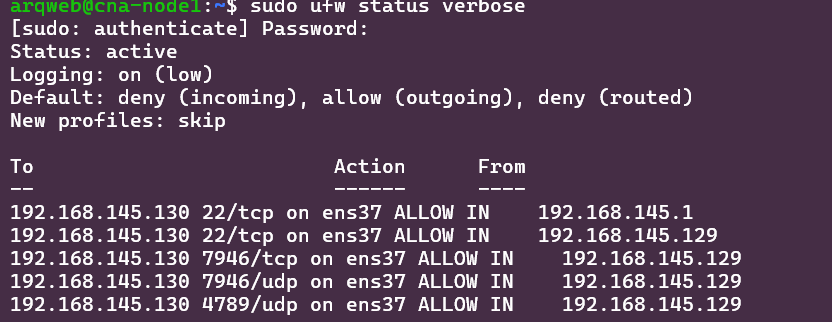
\includegraphics[width=\textwidth,height=5.5cm,keepaspectratio]{../../../cna/docs/evidencias/fase6/preparacion/F6-E2-ufw-vm2.png}
\caption{F6-E2 / P34, VM-2: estado final sin reglas Anywhere; SSH administrativo y Swarm por origen.}
\label{fig:F6-E2-vm2}
\end{figure}

\clearpage
\subsubsection{Resolución local, certificado y continuidad del monolito}
\begin{sloppypar}
En el archivo hosts de Windows se configuraron ambos nombres hacia
\texttt{192.168.145.129}. Se reemitió el certificado X.509 local conservando
la clave privada en VM-1 y una copia del certificado anterior. El nuevo SAN
contiene dos entradas DNS: \path{bookstack.local} y \path{api.bookstack.local}.
Se validó la configuración de Nginx antes de recargarla.
\end{sloppypar}

\begin{figure}[H]
\centering

\includegraphics[width=\textwidth]{../../../cna/docs/evidencias/fase6/preparacion/PRE-B1-hosts-dos-dominios.png}
\caption{Resolución en Windows: ambos nombres apuntan a la interfaz privada de VM-1.}
\label{fig:b1-hosts}
\end{figure}
\begin{figure}[H]
\centering
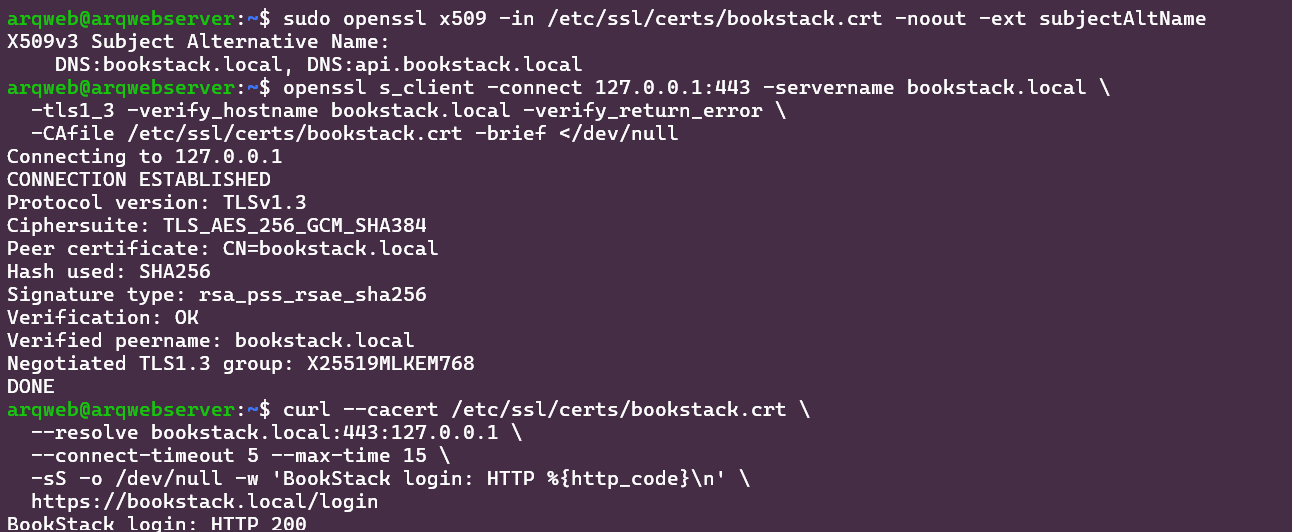
\includegraphics[width=\textwidth,height=11cm,keepaspectratio]{../../../cna/docs/evidencias/fase6/preparacion/F6-E3-certificado-doble-san.png}
\caption{F6-E3 / P35: doble SAN, negociación TLS 1.3 con Verification: OK y login de BookStack con HTTP 200.}
\label{fig:F6-E3}
\end{figure}

\begin{sloppypar}
La comprobación usa \texttt{--cacert} y \texttt{-CAfile} con el certificado
local, sin desactivar la validación mediante \texttt{curl -k}. No demuestra
por sí sola que Windows confíe en el certificado. El integrante también
confirmó la comprobación del nombre \texttt{api.bookstack.local}; la captura
incorporada documenta en detalle \texttt{bookstack.local}. El dominio API
y su SAN quedan preparados; el server block y las rutas \texttt{/v2/}
corresponden a B5 y aún no se declaran implementados.
\end{sloppypar}

\clearpage
\subsubsection{Cierre de B1 y trazabilidad}
\begin{table}[H]
\centering\small
\begin{tabularx}{\textwidth}{>{\raggedright\arraybackslash}p{2.2cm}X>{\raggedright\arraybackslash}p{3cm}}
\toprule
\textbf{Requisito} & \textbf{Resultado documentado} & \textbf{Referencia} \\
\midrule
Clon y recursos & VM-2 enlazada, con hostname/IP propios y recursos registrados. & Tabla \ref{tab:b1-recursos}; figuras \ref{fig:b1-clon-enlazado}--\ref{fig:b1-vm2-creada}. \\
Docker y clúster & Engine y Compose en ambos nodos; dos nodos Ready. & F6-E1 / P33; figuras \ref{fig:b1-docker-vm1}--\ref{fig:F6-E1}. \\
Política UFW & Swarm por origen privado; worker sin reglas generales de acceso. & F6-E2 / P34; figuras \ref{fig:F6-E2-vm1} y \ref{fig:F6-E2-vm2}. \\
Hosts y X.509 & Ambos nombres hacia VM-1; certificado con dos DNS en SAN. & F6-E3 / P35; figuras \ref{fig:b1-hosts} y \ref{fig:F6-E3}. \\
Continuidad & Login del monolito responde HTTP 200 con validación TLS. & Figura \ref{fig:F6-E3}. \\
\bottomrule
\end{tabularx}
\caption{Trazabilidad del cierre de infraestructura B1.}
\label{tab:b1-cierre}
\end{table}

\textbf{Resultado: infraestructura de B1 preparada para continuar con B2.}
No se confunde este cierre con el despliegue de los microservicios ni con
los criterios globales de la Fase 6. Quedan asociados a B3/B5 el presupuesto
real de memoria bajo carga y el filtrado efectivo de los puertos Docker
que se publiquen. Un único manager y un único worker no aportan alta
disponibilidad ante la pérdida de cualquiera de estos nodos.

Las salidas de UFW no prueban automáticamente el filtrado de los puertos
publicados por Docker. Al desplegarlos se comprobarán las reglas efectivas
y el rechazo desde un origen no autorizado.

Las salidas y capturas originales se conservan en el repositorio. Los
scripts de instalación, configuración del worker y renovación del
certificado se encuentran en \path{cna/deploy/scripts/}. No se incluyen
claves privadas, tokens Swarm ni archivos de respaldo con secretos en el
informe o en el control de versiones.
